\chapter{La misión de búsqueda, pieza por pieza}
\label{cap:mision}

\begin{enpocas}
Cómo está programada la misión (\cod{mision_node}): el barrido, la re-observación de candidatas dudosas
(Algoritmo~1), el cambio a la red neuronal con la consigna adelantada, los avisos GPS, la evasión y las
métricas que se guardan al final.
\end{enpocas}

\section{El ciclo}

La misión corre a 20~Hz. En cada ciclo publica una consigna de posición (\cod{TrajectorySetpoint} en
NED) y el modo \emph{offboard}; tras el primer segundo pide a PX4 cambiar a offboard y armar.

\begin{description}
  \item[Despegue:] sube a la vertical del origen hasta la altura de trabajo (30~m).
  \item[Barrido:] recorre las franjas. La consigna avanza a 3~m/s sin alejarse más de 3~m del
        vehículo (\cod{adelanto_max}).
  \item[Re-observación] (\cod{estrategia:=reobs}): al terminar cada franja, si hay candidatas dudosas
        (confianza entre $s_1 = 0.3$ y $s_2 = 0.6$), va a la más cercana: baja a 20~m, con un
        desplazamiento lateral de 6~m para verla desde otro ángulo, espera 3~s y regresa. Cada candidata
        se re-observa a lo más dos veces (Algoritmo~1).
  \item[Aterrizaje:] al terminar, devuelve el control al piloto (si volaba la red) y aterriza.
  \item[Fin:] calcula las métricas, escribe el JSON y termina; el \emph{launch} se cierra solo.
\end{description}

\section{Con la red neuronal}

Con \cod{controlador:=red}, al llegar a la altura de trabajo la misión cambia al modo \emph{Neural
Control} (el identificador lo da PX4 al registrar el modo) y regresa a offboard antes de aterrizar.
Además manda la \textbf{consigna adelantada} $p_{ref} + 1.6\,v_{ref}$ (1.25 en vertical), que convierte
a la red ---que imita una PD--- en una PD con prealimentación (capítulo~\ref{cap:control-neuronal}). El
registro guarda la consigna sin adelanto.

\begin{leccion}
Se probó suavizar el adelanto con un filtro de 1~s para que en las esquinas la consigna no saltara
4.8~m de lado. Empeoró: el adelanto filtrado seguía apuntando en la dirección vieja y el dron se pasaba
de la esquina (RMSE de la ruta de 0.23 a 0.37~m). Sin filtro es exactamente una PD con prealimentación;
el filtro quedó como opción (\cod{tau_adelanto}) desactivada.
\end{leccion}

\section{Avisos con GPS}

Cuando una candidata se confirma durante el barrido ---confianza acumulada $\ge 0.6$, al menos 10
detecciones fusionadas, dentro del área y a más de 5~m de las ya avisadas--- la misión publica una sola
vez:
\begin{itemize}
  \item \cod{/personas/gps}: \cod{NavSatFix} con latitud, longitud y altitud (\cod{frame_id}
        \cod{persona_k});
  \item \cod{/personas/alerta}: el texto del aviso;
\end{itemize}
ambos con QoS \emph{transient local} (quien se suscriba tarde también los recibe). Además lo escribe en la
terminal y en \cod{~/personas_localizadas.csv}:
\begin{lstlisting}
PERSONA 2 LOCALIZADA 2026-10-23 07:50:56
  GPS: 19.482212, -99.245049  (19°28'55.9"N 99°14'42.2"W)
  Mapa: https://www.google.com/maps?q=19.482212,-99.245049
  Local: (-40.0, 35.2) m   confianza 1.00, 10 detecciones
\end{lstlisting}
y en el JSON del mapa que dibuja MAVProxy.

\begin{figure}[H]
\centering
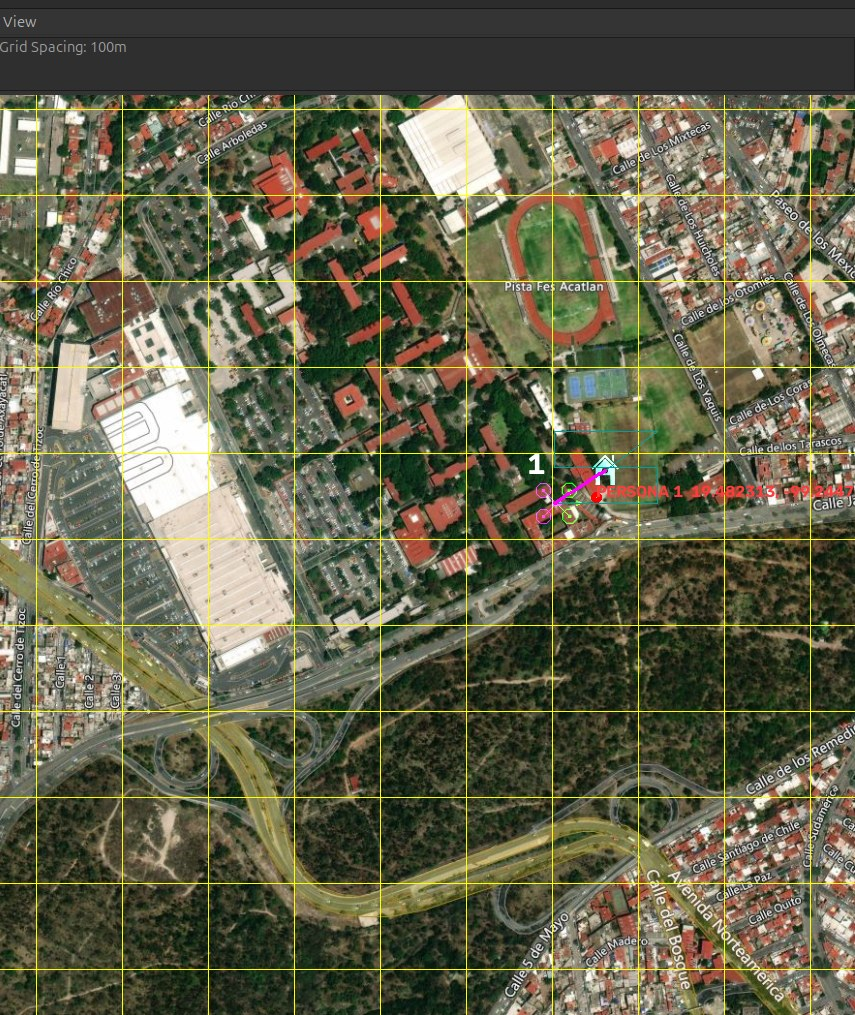
\includegraphics[width=0.55\textwidth]{mapa_personas.jpg}
\caption{El mapa de MAVProxy durante una misión: la persona 1 marcada con sus coordenadas.}
\end{figure}

\begin{leccion}
La primera versión avisó 8 veces para 3 personas: una vista durante el despegue (con 5~m de error),
dos a 250~m (rayos casi horizontales en las vueltas) y otras en grupos de robles. Se agregaron tres
filtros: solo durante el barrido, solo dentro del área y el límite de 60° en el localizador. Quedaron 4 a
6 avisos para 3 personas: las falsas alarmas persistentes de los robles alcanzan las mismas 10
detecciones que las personas reales, así que subir el umbral no las separa. Resolverlas toca al detector
o a la re-observación.
\end{leccion}

\section{Evasión de obstáculos}

Los puntos del LiDAR pasan al marco del mundo con la pose estimada por el piloto (convertida de NED-FRD
a ENU-FLU), se descartan los del suelo y se guardan los cercanos. Si el tramo recto hacia el siguiente
punto pasa a menos de 3~m de un obstáculo a la altura del dron, la consigna toma el rumbo libre más
cercano o sube (\cod{mision/evasion.py}, el mismo algoritmo del capítulo anterior). A 30~m sobre copas de
6.5~m no actúa durante el barrido: protege los tramos bajos y cualquier cambio de altura o de bosque.

\section{Métricas}

Al terminar, la misión compara las candidatas con la verdad (\cod{metricas.py}) y guarda en el JSON:
\begin{longtable}{>{\raggedright\arraybackslash}p{5cm}p{10cm}}
\toprule
\cod{personas_localizadas} & personas con una candidata detectada a menos de 5~m (asignación uno a uno) \\
\cod{falsas_alarmas} & candidatas detectadas que no corresponden a nadie \\
\cod{error_localizacion_m} & distancia media entre persona y candidata \\
\cod{rmse_seguimiento} & distancia RMS del dron a la ruta durante el barrido (sin los desvíos) \\
\cod{reobservaciones}, \cod{duracion_s} & desvíos hechos y duración \\
\cod{por_min_detecciones} & lo mismo exigiendo 1, 3, 5 o 10 detecciones fusionadas \\
\cod{avisos}, \cod{trayectoria}, \cod{eventos} & avisos GPS, trayectoria a 25~Hz y cambios de estado \\
\bottomrule
\end{longtable}
